\documentclass[english,12pt,a4paper,pdftex]{article}

%% Nämä komennot asettavat oikean tekstiencodauksen.
\usepackage[utf8]{inputenc}
\usepackage[OT1]{fontenc}

\usepackage{natbib}

\bibpunct{(}{)}{;}{a}{,}{,}

\usepackage{verbatim}

%% Tämä paketti on pakollinen
%% Valitse korkeakoulusi näistä: arts, biz, chem, elec, eng, sci.
%%
%% This package is required
%% Choose your school from arts, biz, chem, elec, eng, sci.
\usepackage[sci]{aaltothesis}

%% Jos käytät latex-komentoa käännettäessä (oletusarvo) 
%% kuvat kannattaa tehdä eps-muotoon. Älä käytä ps-muotoisia kuvia!
%% Käytä seuraavaa latex-komennon ja eps-kuvien kanssa 
%%
%% Jos tääs käytät pdflatex-komentoa, joka kääntää tekstin suoraan
%% pdf-tiedostoksi, kuvasi on oltava jpg-formaatissa tai pdf-formaatissa.
%%
%% Use this if you run pdflatex and use jpg/pdf-format pictures.
%%
\usepackage{graphicx}

%% Saat pdf-tiedoston viittaukset ja linkit kuntoon seuraavalla paketilla.
%% Paketti toimii erityisen hyvin pdflatexin kanssa. 
%%
%% Use this if you want to get links and nice output with pdflatex
%\usepackage[pdfpagemode=None,colorlinks=true,urlcolor=red,%
%linkcolor=blue,citecolor=black,pdfstartview=FitH]{hyperref}

%% Jos et jostain syystä tykkää käyttää
%% edellistä hyperref pakettia, voit käyttää myös seuraavaa pakettia
%% (tarvitaan lähinnä url-komennon määrittämiseen ja formatoimiseen)
%%
%% Use this if you do not like hyperref package - this
%% defines url environment and formats it correctly
\usepackage{url}

%% Matematiikan fontteja, symboleja ja muotoiluja lisää, näitä tarvitaan usein 
%%
%% Use this if you write hard core mathematics, these are usually needed
% \usepackage{amsfonts,amssymb,amsbsy}  

%% Vaakasuunnan mitat, ÄLÄ KOSKE!
\setlength{\hoffset}{-1in}
\setlength{\oddsidemargin}{35mm}
\setlength{\evensidemargin}{25mm}
\setlength{\textwidth}{15cm}
%% Pystysuunnan mitat, ÄLÄ KOSKE!
\setlength{\voffset}{-1in}
\setlength{\headsep}{7mm}
\setlength{\headheight}{1em}
\setlength{\topmargin}{25mm-\headheight-\headsep}
\setlength{\textheight}{23cm}


%% Kaikki mikä paperille tulostuu, on tämän jälkeen
%%
%% Output starts here
\begin{document}

%% Korjaa vastaamaan korkeakouluasi, jos automaattisesti asetettu nimi on 
%% virheellinen 
%%
%% Change the school field to describe your school if the autimatically 
%% set name is wrong
% \university{aalto University}{aalto-Yliopisto}
% \school{School of Electrical Engineering}{SähköTekniikan korkeakoulu}

%% Vain kandityölle: Korjaa seuraavat vastaamaan koulutusohjelmaasi
%%
%% Only for B.Sc. thesis: Choose your degree programme. 
% \degreeprogram{Electronics and electrical engineering}% {Elektroniikka ja sähkötekniikka}
%%

%% Vain DI/M.Sc.- ja lisensiaatintyölle: valitse laitos, 
%% professuuri ja sen professuurikoodi. 
%%
%% Only for M.Sc. and Licentiate thesis: Choose your department,
%% professorship and professorship code. 
\department{TODO: Department of Radio Science and Technology}
{Radiotieteen ja -tekniikan laitos}
\professorship{Circuit theory}{Piiriteoria}
\code{T-123}
%%

%% Valitse yksi näistä kolmesta
%%
%% Choose one of these:
%\univdegree{BSc}
\univdegree{MSc}
%\univdegree{Lic}

%% Oma nimi
%%
%% Should be self explanatory...
\author{Mikko Koski}

%% Opinnäytteen otsikko tulee vain tähän. Älä tavuta otsikkoa ja
%% vältä liian pitkää otsikkotekstiä. Jos latex ryhmittelee otsikon
%% huonosti, voit joutua pakottamaan rivinvaihdon \\ kontrollimerkillä.
%% Muista että otsikkoja ei tavuteta! 
%% Jos otsikossa on ja-sana, se ei jää rivin viimeiseksi sanaksi 
%% vaan aloittaa uuden rivin.
%% 
%% Your thesis title. If the title is very long and the latex 
%% does unsatisfactory job of breaking the lines, you will have to
%% break the lines yourself with \\ control character. 
%% Do not hyphenate titles.
\thesistitle{Effective communication media for customer feedback in agile software projects}{Tehokkaat kommunikaatiokanavat asiakaspalautteen antamiseen ketterissä ohjelmistoprojekteissa}

\place{Espoo}
%% Kandidaatintyön päivämäärä on sen esityspäivämäärä! 
%% 
%% For B.Sc. thesis use the date when you present your thesis. 
\date{20.3.2012}

%% Kandidaattiseminaarin vastuuopettaja tai diplomityön valvoja.
%% Huomaa tittelissä "\" -merkki pisteen jälkeen, 
%% ennen välilyöntiä ja seuraavaa merkkijonoa. 
%% Näin tehdään, koska kyseessä ei ole lauseen loppu, jonka jälkeen tulee 
%% hieman pidempi väli vaan halutaan tavallinen väli.
%%
%% B.Sc. or M.Sc. thesis supervisor 
%% Note the "\" after the comma. This forces the following space to be 
%% a normal interword space, not the space that starts a new sentence. 
\supervisor{Prof.\ Tapio Takala}{Prof.\ Tapio Takala}

%% Kandidaatintyön ohjaaja(t) tai diplomityön ohjaaja(t)
%% 
%% B.Sc. or M.Sc. thesis advisors(s). 
%%
%% Note that there has been a change in the official EN translation
%% of the Finnish title ``ohjaaja'' which in the previous version (1.5) 
%% of this document was called ``instructor''. The recommended
%% translation is now ``advisor''.  
%% However, the LaTeX internal variable remains \instructor
%% as there is little point to change the variable name. 
%%
%\instructor{Prof. Pirjo Professori}{Prof. Pirjo Professori}
\instructor{Risto Sarvas}{Risto Sarvas}
%\instructor{M.Sc.\ (Tech.) Polli Pohjaaja}{DI Polli Pohjaaja}

%% Aaltologo: syntaksi:
%% \uselogo{aaltoRed|aaltoBlue|aaltoYellow|aaltoGray|aaltoGrayScale}{?|!|''}
%% Logon kieli on sama kuin dokumentin kieli
%%
%% Aalto logo: syntax:
% \uselogo{aaltoRed|aaltoBlue|aaltoYellow|aaltoGray|aaltoGrayScale}{?|!|''}
%% Logo language is set to be the same as the document language.
\uselogo{aaltoRed}{''}

%% Tehdään kansilehti
%%
%% Create the coverpage
\makecoverpage


%% Suomenkielinen tiivistelmä
%% 
%% Finnish abstract
%%
%% Tiivistelmän avainsanat
\keywords{Avainsanoiksi valitaan kirjoituksen sisältöä keskeisesti kuvaavia
käsitteitä}
%% Tiivistelmän tekstiosa
\begin{abstractpage}[finnish]
  Tiivistelmässä on lyhyt selvitys (noin 100 sanaa)
  kirjoituksen tärkeimmästä sisällöstä: mitä ja miten on tutkittu,
  sekä mitä tuloksia on saatu. 
  Tiivistelmässä on lyhyt selvitys (noin 100 sanaa)
  kirjoituksen tärkeimmästä sisällöstä: mitä ja miten on tutkittu,
  sekä mitä tuloksia on saatu. 

  Tiivistelmässä on lyhyt selvitys (noin 100 sanaa)
  kirjoituksen tärkeimmästä sisällöstä: mitä ja miten on tutkittu,
  sekä mitä tuloksia on saatu. 
  Tiivistelmässä on lyhyt selvitys (noin 100 sanaa)
  kirjoituksen tärkeimmästä sisällöstä: mitä ja miten on tutkittu,
  sekä mitä tuloksia on saatu. 
  Tiivistelmässä on lyhyt selvitys (noin 100 sanaa)
  kirjoituksen tärkeimmästä sisällöstä: mitä ja miten on tutkittu,
  sekä mitä tuloksia on saatu. 
\end{abstractpage}

%% Pakotetaan uusi sivu varmuuden vuoksi, jotta 
%% mahdollinen suomenkielinen ja englanninkielinen tiivistelmä
%% eivät tule vahingossakaan samalle sivulle
%%
%% Force new page so that English abstract starts from a new page
\newpage
%
%% English abstract, uncomment if you need one. 
%% 
%% Abstract keywords
\keywords{Resistor, Resistance,\\ Temperature}
%% Abstract text
\begin{abstractpage}[english]
 Your abstract in English. Try to keep the abstract short, approximately 
 100 words should be enough. Abstract explains your research topic, 
 the methods you have used, and the results you obtained.  
\end{abstractpage}
%% Note that 
%% if you are writting your master's thesis in English place the English
%% abstract first followed by the possible Finnish abstract

%% Esipuhe 
%%
%% Preface
\mysection{Preface}
TODO: Haluan kiittää Professori Pirjo 
Professoria ja ohjaajaani Olli Ohjaajaa hyvästä ja 
huonosta ohjauksesta.\\

\vspace{5cm}
Otaniemi, 9.3.2012

\vspace{5mm}
{\hfill Mikko Koski \hspace{1cm}}

%% Pakotetaan varmuuden vuoksi esipuheen jälkeinen osa
%% alkamaan uudelta sivulta
%%
%% Force new page after preface
\newpage


%% Sisällysluettelo
%% addcontentsline tekee pdf-tiedostoon viitteen sisällysluetteloa varten
%% 
%% Table of contents. 
%\addcontentsline{toc}{section}{Sisällysluettelo}
\addcontentsline{toc}{section}{Contents}
%% Tehdään sisällysluettelo
%%
%% Create it. 
\tableofcontents


%% Symbolit ja lyhenteet
%%
%% Symbols and abbreviations
% \mysection{Symbolit ja lyhenteet}
% \mysection{Symbols and abbreviations}

% \subsection*{Lyhenteet}

\clearpage

\subsection*{Abbreviations}

\begin{tabular}{ll}
MRT         & Media Richness Theory \\
MST         & Media Synchronocity Theory \\
API         & Application Programming Interface
\end{tabular}


%% Sivulaskurin viilausta opinnäytteen vaatimusten mukaan:
%% Aloitetaan sivunumerointi arabialaisilla numeroilla (ja jätetään
%% leipätekstin ensimmäinen sivu tyhjäksi, 
%% ks. alla \thispagestyle{empty}).
%% Pakotetaan lisäksi ensimmäinen varsinainen tekstisivu alkamaan 
%% uudelta sivulta clearpage-komennolla. 
%% clearpage on melkein samanlainen kuin newpage, mutta 
%% flushaa myös LaTeX:n floatit 
%% 
%% Corrects the page numbering, there is no need to change these
\cleardoublepage

\storeinipagenumber
\pagenumbering{arabic}
\setcounter{page}{1}

\clearpage

%% Leipäteksti alkaa
%%
%% Text body begins. Note that since the text body
%% is mostly in Finnish the majority of comments are
%% also in Finnish after this point. There is no point in explaining
%% Finnish-language specific thesis conventions in English.
\section{Introduction}

Agile software development in its essence is all about feedback. The core principle of agile development is to have short iterations and deliver a possibly shippable product increment after each iteration \citep{schwaber2009agile}. The delivered product increment enables a possibility for customer to give feedback about the outcome of the iteration and this way direct the development organization to the correct route.

Since the rise of agile software development methods, customer communication and customer collaboration have been taken seriosly and they have been identified as one of the key elements in successful software projects \citep{agilemanifesto}. Also, in previous research it has been shown that a lack of communication and customer involvement is one of the biggest challenges faces by agile teams \citep{korkala2006}.

A lot of research has been conducted about communication is software projects but not so many with the focus on some specific aspect of communication. I believe that customer communication in software projects is a wide subject that includes different types of communication methods in differect situations. For example, the communication required while doing planning is very different from the communication required while customer is givin feedback. Thus, it makes sense to focus on specific area of communication.

Tämä luku vastaa kysymykseen:

\begin{itemize}
\item What's the research problem, bigger phenomenon
\item Why does the problem matter?
\end{itemize}

%% Ensimmäinen sivu tyhjäksi
%% 
%% Leave first page empty
\thispagestyle{empty}



%% Opinnäytteessä jokainen osa alkaa uudelta sivulta, joten \clearpage
%%
%% In a thesis, every section starts a new page, hence \clearpage

\clearpage

\section{Literature}

Vastataan kysymykseen:

\begin{itemize}
\item What has been studied before?
\item What hasn't been studied yet?
\end{itemize}

\subsection{Definitions}

Tässä luvussa esitellään työn kannalta tärkeimmät käsitteet.

\subsubsection{Customer feedback}

\begin{itemize}
\item What does \textit{customer} mean?
\item What does \textit{feedback} mean? Feedback from what?
\end{itemize}

\subsubsection{Effective communication}

\begin{itemize}
\item What does \textit{effective} mean? 
\item What makes communication efective? 
\item What are the properties (in this paper) that make communication efective
\end{itemize}

\subsubsection{Agile software projects}

\begin{itemize}
\item What does \textit{agile} mean in this paper?
\end{itemize}

\subsection{Communication in agile software projects}

\begin{itemize}
\item What has been studied about communication?
\item What has been studied about agile software projects?
\item Why hasn't feedback been studied?
\end{itemize}

\subsection{Media theories}

Tässä luvussa esitellään teoriat, joiden pohjalta arvioidaan kommunikaatiotyökaluja.

Etsitään vastauksia mm. seuraaviin kysymyksiin:

\begin{itemize}
\item Millaisia ominaisuuksia hyvässä kommunikaatiotyökalussa on?
\item Miten näitä ominaisuuksia pystyttäisiin tuomaan mukaan tietokoneavusteiseen kommunikaatiotyökaluun (vai pystyykö)
\end{itemize}

\subsubsection{Media Richness Theory}

\begin{itemize}
\item What's the theory all about?
\item What does the theory say about communication media
\end{itemize}

\subsubsection{Media Synchronicity Theory}

\begin{itemize}
\item What's the theory all about?
\item What does the theory say about communication media
\end{itemize}

\subsubsection{Media Neutralness Theory}

\begin{itemize}
\item What's the theory all about?
\item What does the theory say about communication media
\end{itemize}

\subsection{The nature of feedback communication}

Etsitään vastauksia mm. seuraaviin kysymyksiin:

\begin{itemize}
\item Millaisia erityispiirteitä palautteen antamisella on vrt. muu kommunikaatio
\item Miten nämä erityispiirteet vaikuttavat siihen, millaisia ominaisuuksia kommunikaatiovälineen tulisi tukea.
\end{itemize}

\subsubsection{Feedback communication according to MRT}

\begin{itemize}
\item According to MRT, communication media for feedback conversation should be properties A, B and C
\end{itemize}

\subsubsection{Feedback communication according to MST}

\begin{itemize}
\item According to MST, communication media for feedback conversation should be properties A, B and C
\end{itemize}

\subsubsection{Feedback communication according to MNT}

\begin{itemize}
\item According to MNT, communication media for feedback conversation should be properties A, B and C
\end{itemize}

% \clearpage

\section{Research question}

\subsection{Research question}

\begin{itemize}
\item The research question of this paper is ...
\end{itemize}

\subsection{Objectives}

\begin{itemize}
\item The objectives of this study is ...
\end{itemize}

\subsection{Scope}

\begin{itemize}
\item What's included in this paper
\item What's excluded from this paper
\end{itemize}

% \clearpage

\section{Methods}

\subsection{Literature review}

A literature review is done in order to gather theoretical understanding about properties of effective communication media. In this paper the following communication media theories are included: Media Richness Theory, Media Synchronicity Theory and Media Neutralness Theory. 

Media Richness Theory was selected because blah blah...

Media Synchronicity Theory was selected because blah blah...

Media Neutralness Theory was selected because blah blah...

Other communication media theories, such as blah blah was excluded. The reason for exclusion was blah blah...

\begin{itemize}
\item What were the theories to be included?
\item Why those were included?
\item What other pieces of literature was used?
\item What were the inclusion/exclusion criteria for the other pieces of literature?
\end{itemize}

\subsection{Emprical study - Building a prototype for giving feedback}

\begin{itemize}
\item What's Hannotaatio?
\item What kind of properties does Hannotaatio have, from communication media point-of-view
\item What kind of properties are missing from Hannotaatio, from communication media point-of-view
\end{itemize}

\subsection{Validation prototype with semi-structured interviews}

\begin{itemize}
\item How did I select the people to interview
\item How were the interviews structured
\end{itemize}

% \clearpage

\section{Results}

\subsection{Hannotaatio - A visual website feedback tool}

Tähän yleiskuvaus siitä, mikä on Hannotaatio. Vastaa kysymykseen "millainen prototyypistä sitten loppujen lopuksi tuli?". Käytä Screenshotteja

\subsection{Implemented features}

\subsubsection{Easy installation}

An easy installation of Hannotaatio was one of the main goals for the product. Complex installation process can be a show stopping barrier for users who would like to try new communication tools but are not willing to investment too much effort for the introduction of the tool. Because of that, Hannotaatio's installation process is implemented to be as easy and fast as possible.

The installation of Hannotaatio requires minimal amount of coding and configuration. In the simplest case user does not have to do anything else that copy the seven line code snippet provided in Hannotaatio website to user's own site \citep{hannotaatio}.

For advanced users, there is a possibility to create an API key. The purpose of the API is to collect email addresses of the users show that they can be informed about upcoming updates and down-times.

There is also a possibility for advanced users change the default site capturing settings, e.g. turn on the image capturing. This allows smooth use of Hannotaatio even with private websites that are protected by passwords or firewalls.

\subsubsection{Initiating feedback process}

Before customer can start giving the feedback, two things have to happen. First, customer has to see and try out the production from which the feedback will be given. Second, customer has to initiate the selected communication channel. With the traditional communication tools such as email or telephone, the initiation process requires opening email software and creating a new email message or calling to the feedback receiver.

In Hannotaatio a lot of work has been done to make the initiation of the feedback process as easy as possible. The solution to enable easy initiation of feedback communication channel was to add an "I love feedback" button to the upper right corner of the website from which the feedback will be given. This way the gap between the feedback subject and communication tool is minimal.

\begin{figure}[htb]
\begin{center}
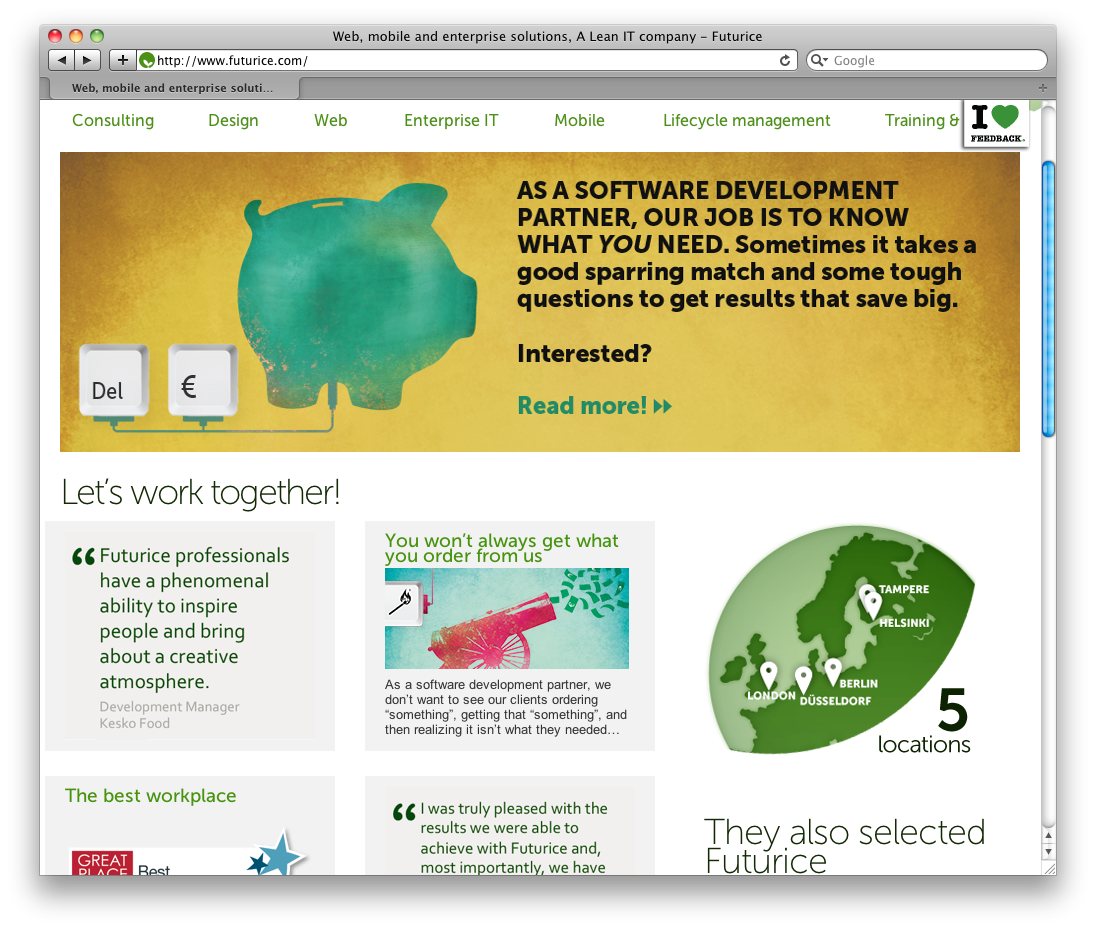
\includegraphics[width=1.0\textwidth]{initiate_feedback.png}
\end{center}
\caption{"I love feedback" button is added to the upper right corner of the website}
\end{figure}

When user presses the "I love feedback" button, a screen capture is taken from the website. After that, user is redirected to an editor, where user is able to draw on top of the captured website.

\subsubsection{Drawing tools}

In Hannotaatio, there are couple of tools for user to draw the feedback on top of the website. The number of tools have been kept minimum on purpose to make the application extremely simple to user.

The available drawing tools are pointing arrow, rectangle and text box. Also, the color of the drawing can be changes between dark and light color scheme. This allows user to draw on top of either light or dark websites.

In requirements gathering phase it was identified that the two most important functions of drawing tools are pointing, highlighting an area and leaving textual note. The three implemented drawing tools allow all the three. However, other drawing tools such as freehand drawing tool or circle drawing tool was left unimplemented, because they we're not critical tools to accomplish the desired functions of pointing, highlighting and leaving a note.

\begin{figure}[htb]
\begin{center}
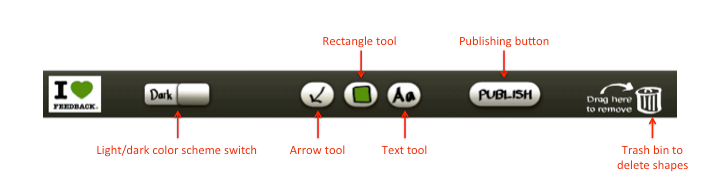
\includegraphics[width=1.0\textwidth]{drawing_tools_annotated_crop.png}
\end{center}
\caption{Hannotaatio toolbar}
\end{figure}

\subsubsection{Sharing the feedback with the team}

When the customer has drawn all the feedback with the available drawing tools, the first step to share the feedback with the team is to publish the feedback by pressing Publish button. When the drawn feedback is published no further modification can be made.

After publishing, user is given a secure URL, which she can share with the team for example via email. The secure URL is randomly generated UUID and it is long enough so that it is impossible to guess. That makes it secure even though viewing the feedback does not require password or any other user credential.

Optionally, if the team has set predefined notification email addresses, a notification email is sent to the team. This happens right after the feedback is published. If notification emails are used, customer does not have to share the secure URL with the team separately.

\subsubsection{Viewing the feedback}

After the drawn feedback has been published by the customer, the development team receives a notification email with the secure URL to the newly drawn feedback or the team receives the secure URL from the customer via email.

The team can now access to the published feedback. Besides seeing the drawn feedback the team can also see when the feedback was given and which browser and operation system was used. Additionally, team is able to access the original site from which the feedback was given by clicking "Go to original page". Also, team or whoever has access to the secure URL and delete the feedback by pressing "Delete" button.

\begin{figure}[htb]
\begin{center}
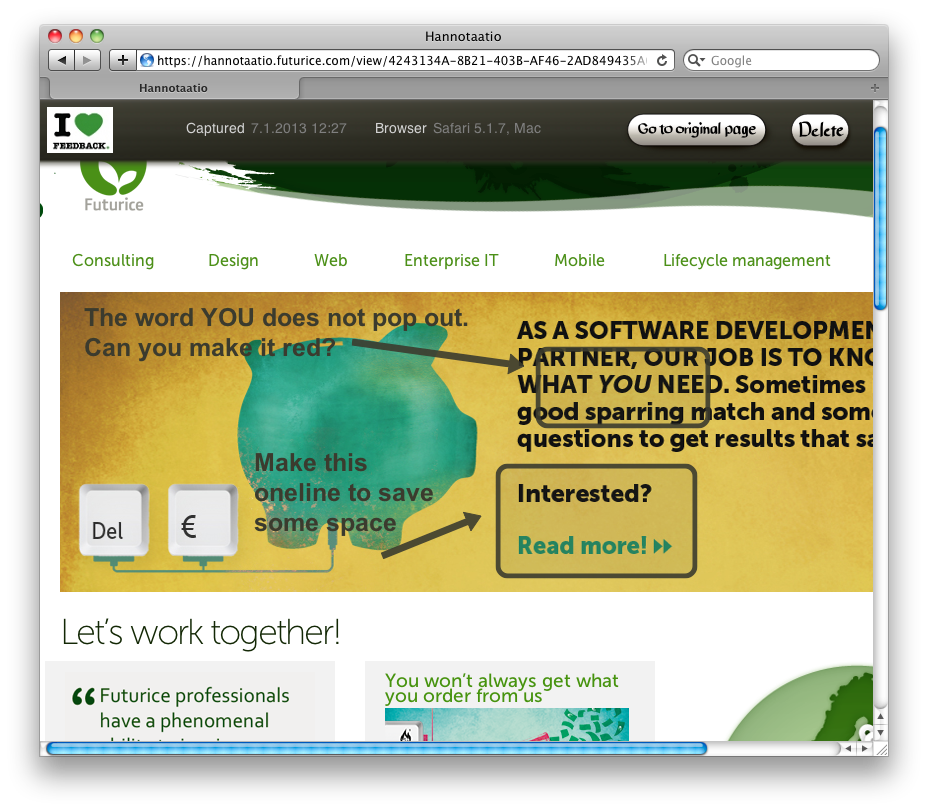
\includegraphics[width=1.0\textwidth]{published_feedback.png}
\end{center}
\caption{Published feedback}
\end{figure}

\subsection{Hannotaatio MRT}

Vastaa kysymykseen: Millainen kommunikaatiotyökalu Hannotaatio on MRT:n mukaan. Sopiiko palautteenantoon?

\subsection{Hannotaatio MST}

As noted in the previous sections, Media Synchronicity Theory identifies the following properties of a communication media: Transmission velocity, parallelism, natural symbol set, rehearsability and reprocessability.

In Hannotaatio the \textbf{transmission velocity} is low. When a developer team has something to show to the customer email is commonly used to notify customer about the new version from which she can give feedback. After the customer has received the notification from a developer team she browses to the site, gives feedback with Hannotaatio and shares the secure URL with the team via email.

The transmission speed of email is instant, but because getting a response to email adds some delay, email is considered to have low transmission velocity. Because there are at least two email send-receive cycles involved in one feedback which is given with Hannotaatio, it can be argued that the transmission velocity for Hannotaatio is rather low.

In Hannotaatio there is a possibility to use notification emails. If notification emails are used, the notification is sent to the team automatically right after the customer has published the feedback. This feature slightly improves the transmission speed because it eliminates one manual email sending from the whole feedback process.

Hannotaatio supports high \textbf{parallelism}. Customer can have many simultaneous feedback conversations at the same time. In the other words this means that customer can give feedback with Hannotaatio at the same time when shes chatting with the team with an instant messaging tool.

Vastaa kysymykseen: Millainen kommunikaatiotyökalu Hannotaatio on MST:n mukaan. Sopiiko palautteenantoon?

Transmission velocity: Matala, mutta tehty parannuksia nopeuttamiseksi

Parallelism: High

Natural symbol set: Matala

Rehearsability: High

Reprocessability: High

\subsection{Hannotaatio MNT}

Vastaa kysymykseen: Millainen kommunikaatiotyökalu Hannotaatio on MNT:n mukaan. Sopiiko palautteenantoon?

\subsection{Hannotaatio, theoretical conclusion}

Edellisissä luvuissa käsiteltiin kutakin teoriaa ja Hannotaatiota erikseen. Tässä luvussa vedetään yhteen.

\subsection{Results of the semi-structured interviews}

Tässä luvussa kerrotaan haastattelujen tulokset.

\begin{itemize}
\item The interviews revealed that property A was very good
\item The interviews revealed that property B was missing and it would have been beneficial.
\end{itemize}

\begin{comment}
Tässä osassa esitetään tulokset ja vastataan tutkielman alussa
esitettyihin tutkimuskysymyksiin. Tieteellisen kirjoitelman
arvo mitataan tässä osassa esitettyjen tulosten perusteella. 

%% Huomaa seuraavassa kappaleessa lainausmerkkien ulkopuolella piste, 
%% koska piste ei lopeta lainattua tekstinpätkää.
%% Jos lainattu tekstinpätkä loppuu välimerkkiin, tulee välimerkki
%% lainausmerkkien sisälle: 
%% "Et tu, Brute?" sanoi Caesar kuollessaan.
Tutkimustuloksien merkitystä on aina syytä arvioida ja tarkastella
kriittisesti.  Joskus tarkastelu voi olla tässä osassa, mutta se
voidaan myös jättää viimeiseen osaan, jolloin viimeisen osan nimeksi
tulee >>Tarkastelu>>. Tutkimustulosten merkitystä voi arvioida myös
>>Johtopäätökset>>-otsikon alla viimeisessä osassa. 

Tässä osassa on syytä myös arvioida tutkimustulosten luotettavuutta.
Jos tutkimustulosten merkitystä arvioidaan >>Tarkastelu>>-osassa,
voi luotettavuuden arviointi olla myös siellä. 

\end{comment}

% \clearpage

\section{Discussion}

\begin{enumerate}
\item What are the weak points of this study?
\item What could be studied in the future?
\end{enumerate}

% \clearpage


\begin{comment}
Tässä osassa selvitetään, mitä tutkimuksen kohteena olevasta
aiheesta tiedetään entuudestaan. Selvityksen tulee kattaa
tasapainoisesti koko tutkimuskenttä. 

Kun opinnäytetyötä kirjoitetaan, on noudatettava 
ohjeita, jotka koskevat opinnäytteen rakennetta,
käytäntöjä, muotoseikkoja sekä ulkoasua. Esitellään näitä
ohjeita tarkemmin.
\end{comment}

%% Osan hienojaottelua alaosiin, eikä välttämättä edes tarpeen,
%% tässä vain esimerkkinä. Käytä harkintasi mukaan
%% osan jaottelua, joskus alaotsikot selventävät asioita ja
%% joskus vain sirpaloittavat tarpeettomasti tekstiä.
%%  Jaottelu menee seuraavasti:
%% \section{osan otsikko} 
%% \subsection{alaotsikko}
%% \subsubsection{ala-alaotsikko}
%% Tätä pitemälle ei pidä jaotella. 
%%
%% Three levels of hierarchy in sectioning should be enough

\begin{comment}
\subsection*{Rakenne}

Opinnäytteen rakenteen tulee olla hyvän tieteellisen
kirjoittamisen käytännön mukainen ja sisältää vähintään seuraavat
osat:

\begin{enumerate}
\item Nimiölehti
\item Tiivistelmä
\item Sisällysluettelo
\item Symboli- ja lyhenneluettelo
\item \label{a} Johdanto
%% Tässä alla on esimerkki lainausmerkkien käytöstä. Suomalaisen tekstin
%% lainausmerkit eivät mene oikein latexissa (tai monissa muissakaan
%% julkaisujärjestelmissä) kun käytetään
%% "-merkkiä, koska latex käyttää amerikkalaista lainausmerkkien
%% tulostustapaa. Vaihtoehtona voi käyttää kulmalainausmerkkejä, jotka
%% myös tulostuvat oikein.
\item  Aikaisempi tutkimus. Työn luonteen niin vaatiessa otsikko voi olla myös
        >>Teoreettinen tausta>>  tai näiden otsikoiden yhdistelmä.
\item Tutkimusaineisto ja -menetelmät %% yhdysmerkki - eli tavuviiva. 
\item Tulokset
\item \label{o} Tarkastelu. Työn luonteen niin vaatiessa otsikko voi
      olla myös >>Johtopäätökset>> tai >>Yhteenveto>> 
      tai edellä mainittujen otsikoiden yhdistelmä.
\item Lähteet
\item Liitteet.
\end{enumerate}

Tiivistelmän ja symboli- sekä lyhenneluetteloiden 
väliin voi sijoittaa halutessaan esipuheen.  

Työn osat \ref{a}-\ref{o} muodostavat \textit{tekstiosan.}  Työn
yksittäisiä osia voidaan jakaa alaotsikoilla alaosiin, joita ei ole
yllä esitetty. Alaotsikoiden käyttäminen selventää parhaimmillaan
tekstiä, ja pahimmillaan sirpaloittaa sitä.  Sirpaloitumista voi estää
huolehtimalla siitä, että samalla sivulla ei esiinny useampaa
alaotsikkoa.  Tekstin jäsentelyssä on yleensä ongelmia, jos osassa on
vain yksi alaosa, tai kirjoittaja joutuu käyttämään useampaa kuin
kahta tasoa (osa ja alaosat): alaosien alaosat ovat harvoin tarpeen.
\subsection*{Sivut ja kirjaintyypit}

Opinnäytteen tulee olla kirjoitettu koneella tai
tekstinkäsittelyohjelmalla yksipuolisesti A4-kokoiselle paperille.
Kandidaatintyön tekstiosan sopiva pituus on noin 15--20 sivua ja
diplomityön noin 60 sivua. Työtä ei ole syytä tarpeettomasti pidentää.

Opinnäytteen tekstiosan kirjaintyypin tulee olla antiikva eli
%% esimerkki pakkotavutuksesta; "serif-tyyppinen" on tavutuksen kannalta
%% hankala, joten pakkotavutetaan se. 
serif\--tyyp\-pi\-nen ja lisäksi kursivoimaton, lihavoimaton sekä kooltaan 12
pistettä (kuten tässä esityksessä). Groteskeja eli \textsf{Sans
  serif}-tyyppisiä kirjaintyyppejä (kuten Helvetica tai Arial) ei saa
käyttää varsinaisessa tekstissä, mutta otsikoissa näitä voidaan
käyttää.  Otsikoissa voidaan käyttää kooltaan edellä mainittua
suurempaa kirjaintyyppiä sekä tyylikeinoja, kuten lihavointia tai
kursivointia.  Tekstissä samantasoisten otsikoiden on kuitenkin oltava
tyyliltään ja kirjainlajeiltaan yhteneväisiä.
%% Esimerkki taulukosta
\begin{table}[htb]
%% Taulukon teksti
\caption{Taulukoissa ja kuvissa kirjaintyypin voi valita
tarkoituksenmukaisesti, mutta kuva- ja taulukkoteksteissä tulee
käyttää samaa kirjaintyyppiä kuin varsinaisessa tekstissä. 
Huomaa taulukon numeroinnin sijoittuminen taulukon yläpuolelle. \label{taulukko1}}
\begin{center}
\fbox{
\begin{tabular}{c|l|r}
\textbf{A} & 1 & $e^{j \omega t}$ \\ \hline
\textsf{B} & 2 & ${\mathfrak R}(c)$ \\ \hline
\texttt{C} & 3 & $ a \in \mathbb{A}$  
\end{tabular}
}
\end{center}
\end{table}

Opinnäytteen vasen marginaali (sidonnan puoli) on
35~mm % tässä ~ muodostaa ns. yhdistävän välilyönnin
ja oikea 25~mm. Ylämarginaali on 25~mm. Leipätekstin korkeus on
enimmillään 230mm. Tämän opinnäytepohjan marginaalien pitäisi olla
paperille tulostettuna oikein, mutta tulostimesta ja paperista
riippuen voi esiintyä yhden tai kahden millimetrin suuruisia eroja.
%% Jos käännät tämän tekstin pdflatex-komennolla ja tulostat sen katselu-
%% ohjelmasta, toteat todennäköisesti em. mittojen poikkeavan enemmän
%% kuin 1-2 mm. 
%% Tämä on seurausta pdf-tiedoston erilaisesta kirjaintyyppimäärityksestä.
%% Korkeatasoista painotyötä varten käytä vain latex-komentoa ja 
%% tulosta postscript-muotoon käännetystä tiedostosta. 
\subsection*{Asemointi}

%% Muutos vanhaan ohjeeseen verrattuna: aikaisemmassa ohjeessa
%% kehotettiin käyttämään vasensuora-asettelua, mutta tässä
%% ohjeessa ollaan luovuttu tuosta vaatimuksesta ja siirrytty
%% huoliteltumpaan, painotuotteenomaisempaan suuntaan.  
Tekstiosan tekstissä käytetään kappaleiden erottamiseen sisennystä,
mutta ensimmäistä otsikon, väliotsikon tai muun katkon jälkeistä
kappaletta ei sisennetä. Jos kuva tai muu katko tulee kappaleiden
väliin, suositellaan katkon jälkeisen kappaleen sisentämistä.

Mikäli oikea reuna halutaan tasata, tulee käyttää tavutusta ja lisäksi
tarkistaa, ettei tekstiin jää lukemista häiritseviä pitkiä sanavälejä. Jos
käytät opinnäytteen tekemisessä \LaTeX-järjestelmää, 
tämä asia hoituu automaattisest.

Opinnäytteen riviväli on 1, mikä on myös tämän opinnäytepohjan käytäntö. 
Kappaleiden tulee yleensä olla ainakin kolmen rivin pituisia, mutta
myös liian pitkiä kappaleita tulee välttää.  Tässä opinnäytepohjassa
ei tekstin luonteen vuoksi voida täysin toteuttaa kappaleen pituutta koskevia
vaatimuksia.

Yksittäisiä, kappaleen päättäviä tai aloittavia rivejä sivun alussa
tai lopussa on vältettävä koko työssä, myös luetteloissa ja
liitteissä.

\subsection*{Numerointi}

Opinnäytteen jokainen osa alkaa uudelta sivulta. Alaosa aloittaa uuden
sivun vain edellisen sivun täytyttyä.

Työn osat numeroidaan siten, että johdanto on ensimmäinen numeroitava
osa. Osien numeroinnissa käytetään arabialaisia numeroita.

Nimiölehti, tiivistelmä, esipuhe, sisällysluettelo ja symboli- ja
lyhenneluettelo numeroidaan esipuheesta tai tämän puuttuessa 
ensimmäiseltä luettelosivulta alkaen roomalaisin numeroin.

Sivunumerointi alkaa toiselta varsinaiselta tekstisivulta, ja 
sivunumeroinnissa käytetään arabialaisia numeroita.

Lähdeluettelo alkaa uudelta sivulta. Lähdeluettelon sivunumerointi 
jatkuu viimeisestä tekstisivusta.

Jokainen liite alkaa uudelta sivulta. Liitteiden sivunumerointi
jatkuu viimeisestä lähdeluettelon sivusta.

Sivunumero sijoitetaan sivun yläreunaan.

Matemaattiset kaavat numeroidaan arabialaisin
numeroin. Kaavanumerointi ei saa katketa osien välissä (eikä niin
tapahdukaan, jos käytät tätä opinnäytepohjaa). Kaikkia kaavoja ei tarvitse
numeroida, vaan kirjoittaja voi käyttää harkintaa numeroinnin
tarpeellisuudessa.  Liitteissä olevat kaavat numeroidaan siten, että
liitteen ajatellaan muodostavan numeroinnin kannalta itsenäisen ja
yhtenäisen kokonaisuuden. Kaavan numero sijoitetaan oikealle puolelle
alla olevan esimerkin mukaisesti
\begin{equation}
D(xy) = (Dx)y + x(Dy),  \hspace{3em} x,y \in \mathbb{A}.
\end{equation}
%% Kaavojen jälkeen ei yleensä laiteta sisennystä. 
Kaikki kuvat ja taulukot numeroidaan erillisen juoksevan numeroinnin
mukaisesti kuten taulukosta \ref{taulukko1} ja kuvasta \ref{kuva1} käy
ilmi.  Liitteissä olevat kuvat ja taulukot numeroidaan siten, että
liitteen ajatellaan muodostavan numeroinnin kannalta itsenäisen ja
yhtenäisen kokonaisuuden. Liitteissä \ref{LiiteA} ja \ref{LiiteB} on
esimerkkejä kaavojen (kaavat \ref{liitekaava1}--\ref{liitekaava2} tai
kaavat \ref{liitekaava3}--\ref{liitekaava4}), kuvien (kuva
\ref{liitekuva}) ja taulukoiden (taulukko \ref{liitetaulukko})
numeroimisesta.  Liitteet numeroidaan suuraakkosin (esimerkiksi Liite
A, Liite B tai pelkästään A, B).
%% Tässä esimerkki kuva1.pdf -nimisen tiedoston tuomisesta kuvaksi.
%% Komento \inclugraphics[parametrit]{argumentti} tuo kuvan.
%% Komento \centering pakottaa kuvan keskelle. 
%% Komento \caption luo kuvatekstin ja sen numeroinnin
%% Parametrit htb pakottavat kuvan suunnilleen siihen 
%% kohtaan, missä se esiintyy tekstin lähdekoodissa
\begin{figure}[htb]
\centering \includegraphics[height=5cm]{kuva1}
\caption{Tämä on esimerkki numeroidusta kuvatekstistä. \label{kuva1}}
\end{figure}

\subsection*{Lähdeviittausten käyttö} 

\begin{comment}

Lähdeviittaukset tulee tehdä huolellisesti ja johdonmukaisesti
numeroviitejärjestelmän mukaisesti. Numeroviitteet järjestetään
lähdeluetteloon viittausjärjestykseen, mutta jos lähdeluettelo
on hyvin laaja (useita sivuja), järjestetään viitteet pääsanan 
mukaiseen aakkosjärjestykseen. Alaviitejärjestelmää
\footnote{Myöskään alaviitteenä olevia kommentteja \underline{ei} suositella
käytettäviksi.} ei käytetä. 

Viitteen sijoittelussa noudatetaan seuraavia sääntöjä:
Jos viite kohdistuu vain yhteen virkkeeseen tai virkkeen 
osaan, viite \cite{Kauranen} sijoitetaan virkkeen sisään ennen virkettä
päättävää pistettä. Jos taas viite koskee tekstin useampaa
virkettä tai kokonaista kappaletta, sijoitetaan viite kappaleen loppuun 
pisteen jälkeen. \cite{Kauranen} 

\subsection*{Lähdeluettelo} 

Lähdeluettelossa esiintyy tavallisesti seuraavassa esitettäviä
lähteitä, joista on numeroviitejärjestelmässä ilmoitettava
asianomaisessa kohdassa vaaditut tiedot.

%% Esimerkki korostamisesta. Lihavoinnin sijasta on tyylikkäämpää
%% ja luettavampaa käyttää kursiivia.
\textit{Kirjasta} ilmoitetaan seuraavat tiedot:

\begin{itemize}
\item[--]tekijät 
\item[--]julkaisun nimi
\item[--]painos, jos useita
\item[--]kustannuspaikka
\item[--]julkaisija tai kustantaja
\item[--]julkaisuaika
\item[--]mahdollinen sarjamerkintö. 
\end{itemize}

Viitteet \cite{Kauranen}--\cite{Koblitz} ovat esimerkkejä kirjan
esittämisestä lähdeluettelossa. Viite \cite[s.\ 83--124]{Koblitz} on
esimerkki lähdeluettelossa esiintyvän kirjan tiettyjen sivujen
esittämisestä tekstissä.

\textit{Artikkelista} kausijulkaisussa ilmoitetaan seuraavat tiedot:

\begin{itemize}

\item[--]tekijät
\item[--]artikkelin nimi
\item[--]kausijulkaisun nimi
\item[--]julkaisuvuosi
\item[--]kausijulkaisun volyymi tai ilmestymisvuosi
\item[--]kausijulkaisun numero
\item[--]sivut, joilla artikkeli on.
\end{itemize}

Viitteet \cite{bcs}--\cite{Deschamps} ovat esimerkkejä artikkelin
esittämisestä lähdeluettelossa.

\textit{Kokoomateoksen luvusta tai osasta} ilmoitetaan seuraavat tiedot:

\begin{itemize}
\item[--]luvun tai osan tekijät
\item[--]luvun tai osan nimi
\item[--]maininta >>Teoksessa>>
\item[--]koko teoksen toimittajat sekä maininta >>(toim.)>>
\item[--]koko teoksen tai konferenssin nimi
\item[--]konferenssiesitelmän kyseessä ollessa sen pitopaikka ja -aika
\item[--]painos, jos useita
\item[--]kustannuspaikka
\item[--]julkaisija tai kustantaja, jos aihetta tämän ilmoittamiseen on
\item[--]julkaisuaika
\item[--]sivut, joilla luku tai osa on 
\item[--]mahdollinen sarjamerkintä.
\end{itemize}

Viitteet \cite{Sihvola}--\cite{Lindblom} ovat esimerkkejä
kokoomateoksen luvun tai osan esittämisestä lähdeluettelossa. 

\textit{Opinnäytetyöstä} ilmoitetaan seuraavat tiedot:

\begin{itemize}
\item[--]tekijä
\item[--]työn nimi
\item[--]opinnäytetyön tyyppi
\item[--]oppilaitoksen nimi
\item[--]osaston, laitoksen tai ohjelman nimi
\item[--]oppilaitoksen sijaintipaikka
\item[--]vuosiluku.
\end{itemize}

Viitteet \cite{Miinusmaa}--\cite{Lonnqvist} ovat esimerkkejä
opinnäytteen esittämisestä lähdeluettelossa. 

\textit{Standardista} ilmoitetaan seuraavat tiedot:

\begin{itemize}
\item[--]standardin tunnus ja numero
\item[--]standardin nimi
\item[--]painos, mikäli ei ole ensimmäinen
\item[--]julkaisupaikka
\item[--]julkaisija
\item[--]julkaisuvuosi
\item[--]sivumäärä.
\end{itemize}
Viite \cite{sfs} on esimerkki standardin esittämisestä opinnäytteen
lähdeluettelossa. 

\textit{Haastattelusta} ilmoitetaan seuraavat tiedot:

\begin{itemize}
\item[--]haastatellun henkilön nimi
\item[--]haastatellun henkilön arvo tai asema
\item[--]haastatellun henkilön edustama organisaatio
\item[--]organisaation osoite
\item[--]maininta siitä, että kyseessä on haastattelu ja haastattelun
päivämäärä. 
\end{itemize}

Viite \cite{haastattelu} on esimerkki 
haastattelun esittämisestä lähdeluettelossa.

Osa sähköisessä muodossa olevista artikkeleista on saatavissa myös
painettuina. \textit{Vain verkosta saatavissa olevasta artikkelista} esitetään
seuraavat tiedot:

\begin{itemize}
\item[--]tekijät
\item[--]artikkelin nimi
\item[--]kausijulkaisun nimi
\item[--]viestintyyppi
\item[--]laitos tai volyymi
\item[--]kausijulkaisun yksittäistä osaa koskeva merkintä tai numero
\item[--]julkaisuvuosi tai maininta >>Päivitetty>> ja päivitysaika
\item[--]maininta >>Viitattu>> ja viittaamisen ajankohta 
\item[--]maininta >>Saatavissa>> ja URL tai 
        maininta >>DOI>> ja DOI-numero (DOI=Digital Object Identifier).
\end{itemize}

Viitteet \cite{Ribeiro}--\cite{kone} ovat esimerkkejä sähköisessä
muodossa olevan artikkelin esittämisestä opinnäytteen
lähdeluettelossa.  Viitteet \cite{Ribeiro} ja \cite{Stieber} ovat
saatavissa sekä painettuna että verkosta, joten viitteiden esitystapa
mukailee painetun artikkelin viitteen esitystapaa, mutta sen lisäksi
kerrotaan julkaisun olevan verkkolehti ja lehden olevan saatavissa
myös painettuna.  Viite \cite{kone} on saatavissa vain verkosta ja
siitä esitetään yllä vaaditut tiedot.

Valitettavasti sähköisessä muodosssa olevasta artikkelista ei ole aina 
saatavissa lai\-tos-, volyymi- tai numerotietoja.

\textit{Sähköisessä muodossa olevasta opinnäytetyöstä} ilmoitetaan
seuraavat tiedot:
 
\begin{itemize}
\item[--]tekijä
\item[--]työn nimi
\item[--]viestintyyppi
\item[--]opinnäytetyön tyyppi
\item[--]oppilaitoksen nimi
\item[--]osaston, laitoksen tai ohjelman nimi
\item[--]oppilaitoksen sijaintipaikka
\item[--]vuosiluku
\item[--]viittamisen ajankohta
\item[--]maininta >>Saatavissa>> ja URL tai 
        maininta >>DOI>> ja DOI-numero.
\end{itemize}

Viite \cite{Adida} on esimerkki sähköisessä muodossa olevan
opinnäytteen esittämisestä lähdeluettelossa.

Viite \cite{viittaaminen} on esimerkki itsenäisen kirjoituksen sisältävästä
verkkosivusta. Tällainen lähde on rinnastettavissa erillisteokseen.
\textit{Verkkosivusta} esitetään tiedot:

\begin{itemize}
\item[--] tekijät
\item[--] otsikko
\item[--] maininta >>Päivitetty>> ja päivitysaika 
\item[--] maininta >>Viitattu>> ja viittaamisen ajankohta
\item[--] Maininta >>Saatavissa>> ja URL.
\end{itemize}

Joskus verkkosivun kirjoitus on jaettu useammalle sivulle, jolloin
lähdeluetteloon kirjataan vain sellainen verkko-osoite, joka koskee
koko kirjoitusta tai sen etusivua, ellei sitten 
todella tarkoiteta kirjoituksen yksittäistä sivua. 

\subsection*{Muuta huomioitavaa lähdeluettelossa}

%% Muutos vanhoihin ohjeisiin koskien kieltä.
Lähdeluettelossa työn ja julkaisun nimi kirjoitetaan alkuperäisessä
muodossaan. Julkaisijan kotipaikka kirjoitetaan alkukielisessä
muodossaan.

Viittamista koskevassa suomalaisessa standardissa
SFS 5342 \cite{sfs} vaaditaan julkaisuista ilmoitettavaksi myös ISBN- tai
ISSN-numerot, mutta näissä opinnäyteohjeissa ei ISBN- ja 
ISSN-numeroita vaadita. 

\end{comment}

%% Lähdeluettelo
\bibliographystyle{plainnat}
\bibliography{ref}

%% Liitteet 
\appendix 

\clearpage

\begin{comment}
\addcontentsline{toc}{section}{Liite A}
\section{Esimerkki liitteestä\label{LiiteA}}
%% Liitteiden kaavat, taulukot ja kuvat numeroidaan omana kokonaisuutenaan
%%
%% Equations, tables and figures have their own numbering in Appendices
\renewcommand{\theequation}{A\arabic{equation}}
\setcounter{equation}{0}  
\renewcommand{\thefigure}{A\arabic{figure}}
\setcounter{figure}{0}
\renewcommand{\thetable}{A\arabic{table}}
\setcounter{table}{0}

Liitteet eivät ole opinnäytteen kannalta välttämättömiä ja 
opinnäytteen tekijän on 
kirjoittamaan ryhtyessään hyvä ajatella pärjäävänsä ilman liitteitä.
Kokemattomat kirjoittajat, jotka ovat huolissaan
tekstiosan pituudesta, paisuttavat turhan 
helposti liitteitä pitääkseen tekstiosan pituuden annetuissa rajoissa.
Tällä tavalla ei synny hyvää opinnäytettä.   

Liite on itsenäinen kokonaisuus, vaikka se täydentääkin tekstiosaa.
Liite ei siten ole pelkkä listaus, kuva tai taulukko, vaan 
liitteessä selitetään aina sisällön laatu ja tarkoitus. 

Liitteeseen voi laittaa esimerkiksi listauksia. Alla on 
listausesimerkki tämän liitteen luomisesta. 

%% Verbatim-ympäristö ei muotoile tai tavuta tekstiä. Fontti on monospace.
%% Verbatim-ympäristön sisällä annettuja komentoja ei LaTeX käsittele. 
%% Vasta \end{verbatim}-komennon jälkeen jatketaan käsittelyä.
\begin{verbatim}
    \clearpage
	\appendix
	\addcontentsline{toc}{section}{Liite A}
	\section*{Liite A}
	...
	\thispagestyle{empty}
	...
	tekstiä
	...
	\clearpage
\end{verbatim}

Kaavojen numerointi muodostaa liitteissä oman kokonaisuutensa:
\begin{eqnarray}
d \wedge A  &=& F, \label{liitekaava1}\\
d \wedge F  &=& 0. \label{liitekaava2}
\end{eqnarray}


\clearpage
\addcontentsline{toc}{section}{Liite B}
\section{Toinen esimerkki liitteestä\label{LiiteB}}

%% Liitteiden kaavat, taulukot ja kuvat numeroidaan omana kokonaisuutenaan
%%
%% Equations, tables and figures have their own numbering in Appendices
\renewcommand{\theequation}{B\arabic{equation}}
\setcounter{equation}{0}  
\renewcommand{\thefigure}{B\arabic{figure}}
\setcounter{figure}{0}
\renewcommand{\thetable}{B\arabic{table}}
\setcounter{table}{0}

Liitteissä voi myös olla kuvia, jotka
eivät sovi leipätekstin joukkoon:
%% Ympäristön figure parametrit htb pakottavat
%% kuvan tähän, eikä LaTeX yritä siirrellä niitä
%% hyväksi katsomaansa paikkaan. 
%% Ympäristöä center voi käyttää \centering-
%% komennon sijaan
%%
%% Example of a figure, note the use of htb parameters which force
%% the figure to be inserted here
\begin{figure}[htb]
\begin{center}
\includegraphics[height=8cm]{kuva2}
\end{center}
\caption{Kuvateksti, jossa on liitteen numerointi \label{liitekuva}}
\end{figure}
%%
Liitteiden taulukoiden numerointi on kuvien ja kaavojen kaltainen:
\begin{table}[htb]
\caption{Taulukon kuvateksti. \label{liitetaulukko}}
\begin{center}
\fbox{
\begin{tabular}{lp{0.5\linewidth}}
9.00--9.55  & Käytettävyystestauksen tiedotustilaisuus (osanottajat
ovat saaneet sähköpostitse valmistautumistehtävät, joten tiedotustilaisuus
voidaan pitää lyhyenä).\\
9.55--10.00 & Testausalueelle siirtyminen
\end{tabular}}
\end{center}
\end{table}
Kaavojen numerointi muodostaa liitteissä oman kokonaisuutensa:
\begin{eqnarray}
T_{ik} &=& -p g_{ik} + w u_i u_k + \tau_{ik},  \label{liitekaava3} \\
n_i    &=& n u_i + v_i.                        \label{liitekaava4}
\end{eqnarray}

\end{comment}

\end{document}